\chapter{Modelización de la tarea de aprendizaje} \label{ch:tarea_aprendizaje}

\section{Planteamiento del problema} \label{seq:planteamiento_problema}

La tarea de aprendizaje que consideramos es la de \textbf{clasificación de imágenes}, para la cual el uso de redes convolucionales profundas ha supuesto un gran avance. Nos centraremos en modelar redes convolucionales (profundas y no profundas) para clasificar imágenes.

Dado un elemento $X = (\nv{x_1}, \ldots, \nv{x_N})$, donde $\nv{x_i} \in \R^s \ \forall i \in \deltaset{N}$, queremos clasificarlo en alguna de las etiquetas $\mathcal{Y} = \{1, \ldots, Y \} = \deltaset{Y}$. Con esto, podemos ver que los datos de entrada viven en el espacio

\begin{equation}
	\mathcal{X} := \R^s \times \overset{N}{\ldots} \times \R^s = (\R^s)^N.
\end{equation}

Esta representación de los datos de entrada es natural en muchos escenarios. En el caso de las imágenes, podemos considerar cada vector $\nv{x_i}$ como un conjunto de \textit{pixels} de la imagen, en lo que se conoce como parche o \textit{patch}. Por la estructura local de las imágenes, cada parche debería contener un vecindario de \textit{pixels}, es decir, \textit{pixels} adyacentes. Puede ocurrir que los parches no sean disjuntos, o lo que es lo mismo, que existan \textit{pixels} perteneciendo a más de un parche. Las imágenes contienen información en los colores que contiene cada píxel, pero también en su posición. Esto es claro si tenemos en cuenta que permutando aleatoriamente las posiciones de los \textit{pixels} de una imagen, ésta pierde el sentido. Mostramos un ejemplo de ello en la \imgref{img:desordenar_pixeles_repetida_mates}. A esto nos referimos cuando hablamos de estructura local de la imagen. Una forma natural de generar estos parches a partir de las imágenes consiste en tomar $\nv{x_i}$ como la fila o columna $i$-ésima de la imagen.

\begin{figure}[!hbtp]
	\centering
	\ajustarsubcaptions
	\begin{subfigure}[t]{0.45\textwidth}
		\centering
		
\includegraphics[width=0.9\linewidth]{informatica/ejemploperm_normal}
		\caption{Imagen original}
	\end{subfigure}
	\begin{subfigure}[t]{0.45\textwidth}
		\centering
		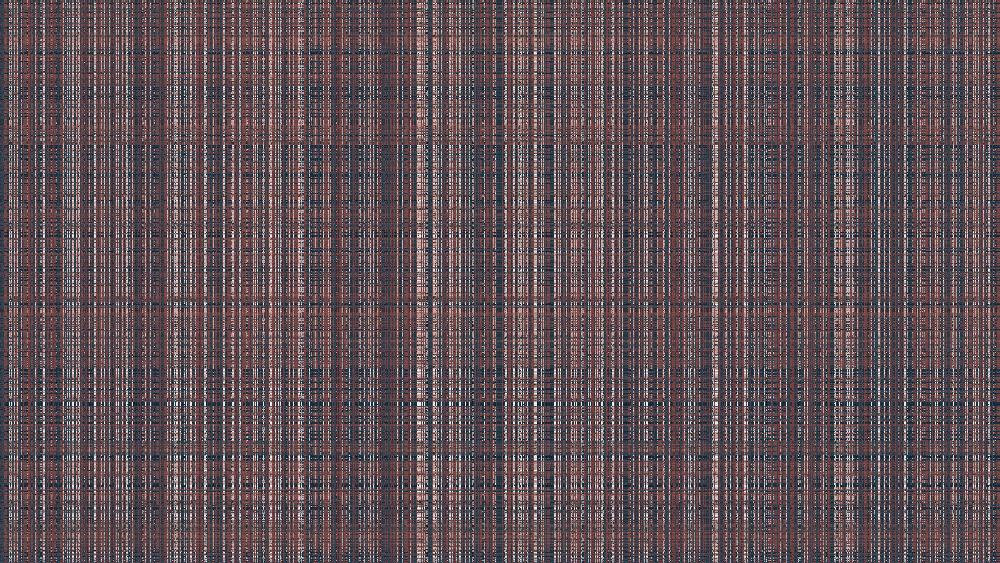
\includegraphics[width=0.9\linewidth]{informatica/ejemploperm_permutada}
		\caption{Imagen original tras aplicar una permutación aleatoria de las posiciones de los \textit{pixels}}
	\end{subfigure}
	\caption{Tenemos que considerar la estructura local de la imagen. La posición de los \textit{pixels} y su vecindario contiene una información fundamental de la que no podemos prescindir. Por tanto, los parches deben contener vecindarios de \textit{pixels}, aunque tengamos distintas estrategias para escoger estos vecindarios.}
	\label{img:desordenar_pixeles_repetida_mates}
\end{figure}

Para decidir la etiqueta de un elemento, consideramos $Y$ \textbf{funciones de puntuación}:

\begin{equation}
	\conjunto{h_y: \mathcal{X} \to \R \dspace / \dspace y \in \mathcal{Y}}.
\end{equation}

\textbf{NOTA PARA JAVIER}: aquí me marcaste debajo de $Y$ y de $\mathcal{Y}$. Escribo $Y$ funciones de puntuación y luego $y \in \mathcal{Y}$ porque he definido $\mathcal{Y} := \deltaset{Y}$. No sé si esta definición aporta poco y lía más que otra cosa, en cuyo caso creo que es mejor quitar la definición de $\mathcal{Y} := \deltaset{Y}$. O si simplemente crees que es mejor que escoja una tipografía o letras que líen menos.
\todo{Borrar esta nota para Javier}

Con esto, dado un elemento $X \in \mathcal{X}$, lo clasificaremos buscando la etiqueta cuya función de puntuación sea máxima, es decir:

$$\hat{y} := \underset{y \in \mathcal{Y}}{argmax} \dspace h_y(X).$$

Por tanto, nuestro \textbf{espacio de hipótesis} es el conjunto de funciones $\Gamma := \conjunto{f: \mathcal{X} \to \R}$. Tanto en la práctica con modelos reales de aprendizaje automático como en nuestras dos modelizaciones, trabajamos en un subconjunto $\tilde{\Gamma} \subseteq \Gamma$ de funciones de puntuación, implementables o bien por el modelo de \textit{machine learning} o bien por nuestra modelización teórica.

\section{Espacio de hipótesis general} \label{sec:espacio_hipotesis_general}
\todo{JMERI: leer de nuevo esta sección completa, porque es muy liosa, repito cosas, introduzco cosas donde no debería. Mirar los contenidos que he borrado}

Nuestro objetivo en esta sección es justificar la elección de las funciones $h_y$ que conformarán el espacio de hipótesis sobre el que trabajaremos. En la \sectionref{sec:repr_funciones_puntuacion} mostramos cuál es la elección final basada en el desarrollo previo. Usaremos ciertos hechos básicos sobre análisis funcional que hemos introducido en la \sectionref{sec:preliminares_funcional}.

\subsection{Planteamiento para construir el espacio de hipótesis} \label{sec:justificacion_func_repr}

Recordemos que los datos de entrada viven en el espacio $\mathcal{X} = (\R^s)^N$ y que, para cada entrada $X \in \mathcal{X}$, tomamos como salida la etiqueta $\hat{y} \in \mathcal{Y}$ que maximice su función de puntuación asociada, que venía dada como:

\begin{equation}
	\hat{y} := \underset{y \in \mathcal{Y}}{argmax} \dspace h_y(X).
\end{equation}

Por lo tanto, buscamos \textbf{construir un espacio de hipótesis} $\mathcal{H} \subseteq L^2((R^s)^N)$ donde elegir nuestras funciones de puntuación. Dicha elección influirá en los modelos de aprendizaje que podamos desarrollar.

Comenzaremos tomando un conjunto de funciones $\conjunto{f_d(\nv{x}): \; d \in \N} \subseteq L^2(\R^S)$ de forma que sea total y linealmente independiente. Llamaremos \textbf{funciones de representación} a las funciones de este conjunto. Gracias a la \propref{prop:conservacion_totalidad_indp_lineal_func_prod} sabemos que la familia de funciones producto inducida $\conjunto{(\nv{x_1}, \ldots, \nv{x_n}) \mapsto \prod_{i = 1}^N f_{d_i}(\nv{x_i}) }_{d_1, \ldots, d_N \in \N} \subseteq L^2((\R^S)^N)$ es también total y linealmente independiente. Por ser total, la \propref{prop:conjuntos_totales_epsilon_aproximacion} nos dice que podemos aproximar funciones de $L^2((\R^S)^N)$ arbitrariamente bien con combinaciones lineales finitas de funciones producto. En la \sectionref{sec:funciones_representacion} hemos visto que podemos escoger funciones de base radial \textit{RBF} o neuronas para tomar un conjunto de funciones de representación que sea total, linealmente independiente y además finito.

\subsection{Representación tensorial}

Con todo lo anterior tenemos $\epsilon$-aproximación a partir de combinaciones lineales finitas de elementos de un conjunto infinito. Vamos a representar esta aproximación con tensores, lo que nos permitirá más tarde trabajar con modelizaciones basadas en descomposiciones tensoriales. Para ello, consideraremos tensores formales $\mathcal{A}^y \in \espaciotensores{N}{\N}$. Esto es, tensores con $N$ modos, cada modo con una dimensión infinita numerable (podemos considerar que tenemos $N$ sucesiones). El papel de estos tensores formales será el de almacenar los coeficientes de la combinación lineal finita dada por la ecuación \eqref{eq:conjuntos_totales_epsilon_aproximacion} y, por lo tanto, los llamaremos \textbf{tensores de coeficientes}. Como esa combinación lineal es finita, nuestro tensor formal tendrá todas las entradas nulas salvo un conjunto finito. Necesitamos usar tensores formales porque tenemos que elegir qué funciones usamos de un conjunto numerable. Y con esto llegamos a:

\begin{equation} \label{eq:hipotesis_en_general}
	h_y(\nv{x_1}, \ldots, \nv{x_N}) \approx \sum_{d_1, \ldots, d_N \in \N} A^y_{d_1, \ldots, d_N} \prod_{i = 1}^N f_{d_i}(\nv{x_i}).
\end{equation}

Como hemos visto que podemos tomar un conjunto de funciones de representación total, linealmente independiente y además finito, es suficiente considerar $\mathcal{A}^y \in \espaciotensores{N}{M}$ para algún $M \in \N$, con lo que el modelo queda:

\begin{equation}
	h_y(\nv{x_1}, \ldots, \nv{x_N}) \approx \sum_{d_1, \ldots, d_N = 1}^{M} \mathcal{A}^y_{d_1, \ldots, d_N} \prod_{i = 1}^N f_{\theta_{d_i}}(\nv{x_i}).
\end{equation}

De esta forma, este modelo será universal. Podemos aproximar arbitrariamente bien cualquier función de puntuación $h_y \in L^2((\R^S)^N)$ con combinaciones lineales, expresadas a partir de la ecuación anterior. Además, como el conjunto de funciones es linealmente independiente, la expresión anterior es única, y nuestro conjunto de funciones actúa de base del espacio. Es decir, una función de puntuación $h_y$ determina únivocamente el tensor de coeficientes $\mathcal{A}^y$, y podemos escribir:

\begin{equation} \label{eq:puntuacion_general}
	h_y(\nv{x_1}, \ldots, \nv{x_N}) = \sum_{d_1, \ldots, d_N = 1}^{M} \mathcal{A}^y_{d_1, \ldots, d_N} \prod_{i = 1}^N f_{\theta_{d_i}}(\nv{x_i}).
\end{equation}

Así, la tarea de aprendizaje consistirá en aprender a partir de los datos de entrenamiento los coeficientes $\theta_1, \ldots, \theta_M$ de las funciones de representación y los tensores de coeficientes $\mathcal{A}^1, \ldots, \mathcal{A}^Y$.

\begin{observacion}
	Usamos la notación $\sum_{d_1, \ldots, d_N = 1}^{M}$ para denotar $\sum_{d_1 = 1}^{M} \sum_{d_2 = 1}^{M} \ldots \sum_{d_N = 1}^{M}$.
\end{observacion}

\subsection{Capa de representación} \label{subs:capa_de_representacion}

En la ecuación \eqref{eq:puntuacion_general} estamos usando las mismas funciones de representación $f_{\theta_1}, \ldots, f_{\theta_M}: \R^s \to \R$ para todas las funciones de puntuación $h_y$. Lo único que cambia entre las distintas funciones de puntuación es el tensor de coeficientes $\mathcal{A}^y$. Nótese además que en la ecuación \refeq{eq:puntuacion_general}, los vectores de entrada $\nv{x_i}$ solo participan en el producto que involucra computar $f_{\theta_{d_i}}(\nv{x_i})$. Por tanto, podemos considerar un paso inicial, que será compartido en los dos modelos que más adelante introduciremos, consistente en computar los valores:

$$\{f_{\theta_d}(\nv{x_i}): \; d \in \deltaset{M},\ i \in \deltaset{N} \}.$$

Una vez que hayamos computado esos $M \cdot N$ valores, ya no necesitamos los vectores $\nv{x_i}$ para nada más. Con esto, es natural considerar que nuestro modelo tenga una primera capa que compute esos valores, a la que llamaremos \textbf{capa de presentación} y que será una capa convolucional con $M$ canales. Por tanto, cada parche de entrada $\nv{x_i} \in \R^s$ acaba siendo representando por un descriptor de longitud $M$. Con esto, en todas las funciones de puntuación los descriptores resultado de la capa de representación serán los mismos. El siguiente diagrama muestra gráficamente cómo actúa la capa de representación, calculando los $N \cdot M$ coeficientes reales que componen los descriptores de dicha capa:

\begin{figure}[!hbtp]
	\centering
	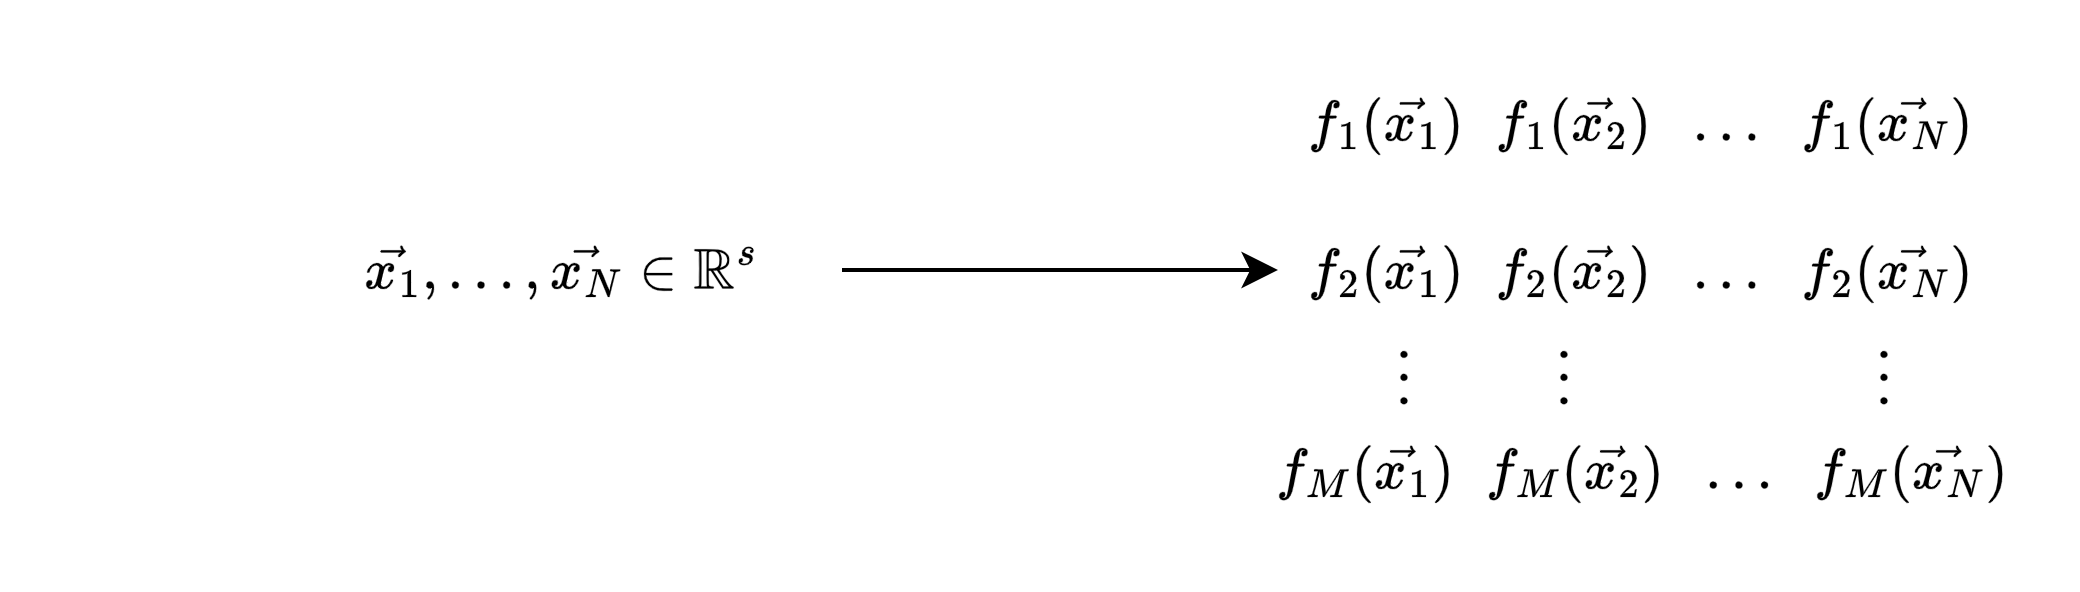
\includegraphics[width=0.8\textwidth]{matematicas/computo_capa_representacion}
	\caption{Ejemplo gráfico sobre cómo actúa la capa de representación. A partir de $N$ parches en $\R^s$, acabamos con $N \cdot M$ coeficientes reales que conformen los descriptores de la capa.}
\end{figure}


\subsection{Ejemplo de cómputo} \label{ejemplo:funcion_puntuacion}

Supongamos que trabajamos con $N = 3, M = 2$. En este caso, una imagen de entrada se compone de los vectores $\nv{x_1}, \nv{x_2}, \nv{x_3} \in \R^s$ (no estamos interesados en el valor de $s \in \N$). Y tenemos dos funciones de representación $f_1, f_2: \R^s \to \R$. El primer paso es computar la capa de representación, que son los $N \cdot M$ coeficientes reales dados por:

\begin{equation}
	\begin{split}
		f_1(\nv{x_1}), f_1(\nv{x_2}), f_1(\nv{x_3}) \\
		f_2(\nv{x_1}), f_2(\nv{x_2}), f_2(\nv{x_3})
	\end{split}
\end{equation}

Y con esto ya podemos expresar nuestra función de puntuación:

\begin{equation}
	\begin{split}
		h_y(\nv{x_1}, \ldots, \nv{x_N}) &= \sum_{d_1, d_2, d_3 = 1}^{2} \mathcal{A}^y_{d_1 d_2 d_3} \prod_{i = 1}^3 f_{d_i}(\nv{x_i}) = A_{111} \; f_1(\nv{x_1}) \; f_1(\nv{x_2}) \; f_1(\nv{x_2}) + A_{112} \; f_1(\nv{x_1}) \; f_1(\nv{x_2}) \; f_2(\nv{x_2}) + \\
		\cdots &+ A_{321} \; f_3(\nv{x_1}) \; f_2(\nv{x_2}) \; f_1(\nv{x_2}) + A_{333} \; f_3(\nv{x_1}) \; f_3(\nv{x_2}) \; f_3(\nv{x_3}).
	\end{split}
\end{equation}

Queda claro que el tensor $\mathcal{A}^y$ contiene los coeficientes que realizan una combinación lineal sobre todos los posibles productos de nuestros $N \cdot M$ valores reales de la capa de representación.

\section{Resumen}

Buscamos resolver una tarea de clasificación de imágenes. Dada una imagen de entrada, debemos asignarle una de las etiquetas $\mathcal{Y} := \{1, \ldots, Y\} = \deltaset{Y}$. Para ello, tomamos la etiqueta cuya función de puntuación asociada $h_y$ sea mayor. Las imágenes de entrada se dividen en parches. Esto es, una imagen viene dada por $N$ vectores $x = (\nv{x_1}, \ldots, \nv{x_N}), \dspace \nv{x_i} \in \R^s \dspace \forall i \in \deltaset{N}$. Elegimos un conjunto finito de funciones de representación que sea total y linealmente independiente. Para ello podemos elegir funciones de base radial \textit{RBF} o neuronas. Aplicando adecuadamente las propiedades del conjunto de funciones, llegamos a la modelización:

\begin{equation}
	h_y(\nv{x_1}, \ldots, \nv{x_N}) = \sum_{d_1, \ldots, d_N = 1}^{M} \mathcal{A}^y_{d_1, \ldots, d_N} \prod_{i = 1}^N f_{\theta_{d_i}}(\nv{x_i}).
\end{equation}

Estudiando esta ecuación nos damos cuenta de que hay un cómputo compartido en todas las funciones de puntuación, que encapsulamos en la capa de representación. Lógicamente, el cómputo de esta capa es compartido para todas las funciones de puntuación.

Las dos arquitecturas que introduciremos más adelante son el resultado de factorizar el tensor de coeficientes $\mathcal{A}^y$ con distintas descomposiciones. Ambas incorporan conceptos claves en la práctica del aprendizaje automático, como la localidad, coeficientes compartidos y \textit{pooling}.
